%Information relative au document
% !TEX encoding = MacOSRoman
\documentclass[a4paper,12pt]{report}


%Paquets
\usepackage[T1]{fontenc}
\usepackage[utf8]{inputenc}
\usepackage[frenchb]{babel}

\usepackage{textcomp}

\usepackage{lmodern}

\usepackage{graphicx}
\usepackage{amsmath}
\usepackage{amsfonts}
%Pour faire un tableau de d\'eriv\'e
\usepackage{tikz,tkz-tab}
\usepackage{float}
\usepackage{here}
\usepackage[left=2cm,right=2cm,top=3cm,bottom=3cm]{geometry}


\renewcommand{\baselinestretch}{1.5}
\makeatletter
\def\@makechapterhead#1{%
  \vspace*{25\p@}%
  {\parindent \z@ \raggedright \normalfont
    \interlinepenalty\@M
    \ifnum \c@secnumdepth >\m@ne
        \Huge\bfseries \thechapter\quad
    \fi
    \Huge \bfseries #1\par\nobreak
    \vskip 20\p@
  }}

\def\@makeschapterhead#1{%
  \vspace*{20\p@}%
  {\parindent \z@ \raggedright
    \normalfont
    \interlinepenalty\@M
    \Huge \bfseries  #1\par\nobreak
    \vskip 20\p@
  }}
\makeatother

%D\'ebut du rapport
\begin{document}

%Page de garde
\title{Rapport \no1 MT12}
\author{Alexandre BALLET et Simon LAURENT}
\date{Printemps 2016}
   
  %  \begin{minipage}{0.4\textwidth}
     % \begin{flushleft} \large
        %\emph{Enseignant :} M. Dajlil Kateb\\
        %\emph{Etablissement : } Universit\'e de Technologie de Compi�\`egne
      %\end{flushright}
    %\end{minipage}
\maketitle

%Table des mati\`eres
\tableofcontents

%Exercice 1
\chapter{S\'erie de Fourier}
	\section{Historique}
		\subsection{Biographie}
Jean-Baptiste Fourier (qu'on connait aussi sous le nom de Joseph Fourier) est n\'e le 21 mars 1768 \`a Auxerre et mort le 16 mai 1830 � Paris. 

En 1794, il est de la premi\`ere promotion de l'\'Ecole Normale Sup\'erieure, o\`u ses professeurs ont pour nom Lagrange, Laplace et Monge. \'El\`eve le plus brillant, il profite de cet excellent entourage pour s'investir beaucoup dans la recherche math\'ematique. En 1797, il remplace Lagrange \`a la chaire d'analyse et de m\'ecanique de l'\'Ecole Polytechnique, bien qu'il n'ait pas encore \`a son actif de d\'ecouverte majeure.

En 1798, il rejoint les exp\'editions napol\'eoniennes en \'Egypte, o\`u de nombreux chercheurs fran\c cais m\`enent d'ambitieuses recherches. Quand Fourier regagne la France en 1801, Napol\'eon n'a pas oubli\'e ses excellents \'etats de service, et le nomme pr\'efet de l'Is\`ere. Il fut un excellent pr\'efet, qui mena \`a bien plusieurs projets d'importance, dont la construction d'une route menant de Lyon � Turin. 

C'est \`a Grenoble que Fourier r\'ealise l'essentiel de ses travaux les plus importants. Son obsession est le probl\`eme de la chaleur, c'est-\`a-dire l'\'etude de l'\'evolution de la temp\'erature d'un corps au cours du temps. De 1802 \`a 1807, il trouve l'\'equation de la propagation de la chaleur dans les corps solides, puis trouve une m\'ethode pour la r\'esoudre, ce qui est maintenant l'analyse de Fourier.

En 1812 Fourier est prim\'e par l'Institut pour son m\'emoire 

En 1817, il est \'elu \`a l'Acad\'emie des sciences r\'ehabilit\'ee. 

En 1822, il devient secr\'etaire de la section math\'ematique. A ce poste, il aidera beaucoup de jeunes math\'ematiciens prometteurs, dont Dirichlet, Sturm ou Ostrogradsky. 
		
		\subsection{Vulgarisation}
		
		L analyse de Fourier consiste en l'\'etude des vibrations \'el\'ementaires des signaux. Supposons que l'on souhaite analyser un signal quelconque, une quantit\'e qui varie \`a mesure que le temps passe : par exemple, le son est fait de l\'eg\`eres variations de pression atmosph\'erique. Au lieu de s'int\'eresser directement aux variations complexes de ce signal, Joseph Fourier eut l'id\'ee de le d\'ecomposer en une combinaison de signaux \'el\'ementaires, dont chacun varie de mani�re tr\`es simple et r\'ep\'etitive : les sinuso\"ides (et leurs fr\`eres jumeaux, les cosinuso\"ides). Chaque sinuso\"ide est caract\'eris\'ee par l'amplitude et la fr\'equence de ses variations. Dans la d�composition de Fourier, les amplitudes nous renseignent sur l'importance relative des fr\'equences correspondantes dans le signal \'etudi\'e.
		
Ainsi les sons qui nous entourent sont faits de la superposition d'une multitude de fr\'equences. La vibration \`a $440$ battements par seconde est un $la$, qui sera per�u avec d'autant plus de puissance que son amplitude est forte. \`A $880$ battements par seconde, on entendra un $la$ de l'octave au-dessus. Si l'on multiplie la fr\'equence par $3$, on passera � la quinte, c'est-\`a-dire au mi, et ainsi de suite. Mais en pratique les sons ne sont jamais purs, ils sont toujours faits de la concomitance de tr\`es nombreuses fr\'equences qui en d\'eterminent le timbre.

Et l'analyse de Fourier sert � tout : \`a analyser les sons et \`a les graver sur un CD, mais aussi \`a analyser les images et \`a les transmettre par Internet, ou \`a analyser les variations du niveau de la mer et \`a pr\'edire les mar\'ees...
Son �grand po�me math�matique� (comme disait Lord Kelvin), enseign\'e dans tous les pays du monde, est utilis\'e chaque jour par des milliards d'humains qui ne s'en rendent m�me pas compte. \\

\begin{center}
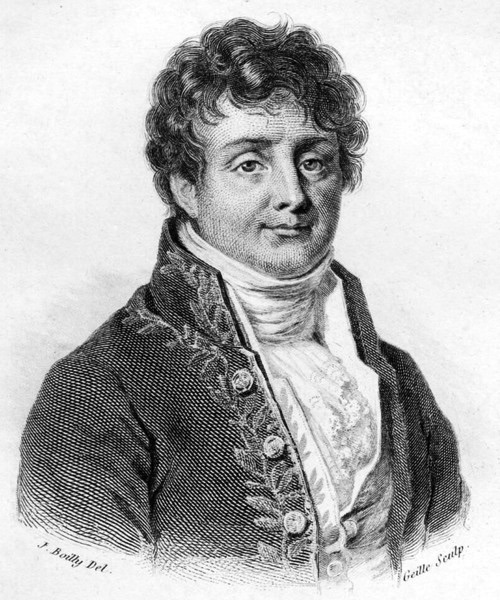
\includegraphics[scale=0.25]{fourier.jpg}\\
\caption{\textit{Joseph Fourier}}
\end{center}



	
	\section{\'Etude de fonctions}
	\begin{enumerate}
		\item $f$ est $2\pi$ p\'eriodique, impaire et vaut $f(x)=1, x \in [0,\pi]$\\
		\begin{enumerate}
			\item Coefficients de Fourier \\ \\
			Les $a(i)$ \'etant nuls. On obtient ainsi les coefficients suivants pour les $b(i)$ : \\ \\
			\begin{centering}
				\begin{tabular}{l l}
					$b(1) = 1.273240$ & \hspace*{2cm}$b(6) = -0.000000$\\
					$b(2) = 0.000000$ & \hspace*{2cm}$b(7) = 0.181891$\\
					$b(3) = 0.424413$ & \hspace*{2cm}$b(8) = 0.000000$\\
					$b(4) = 0.000000$ & \hspace*{2cm}$b(9) = 0.141471$\\
					$b(5) = 0.254648$ & \hspace*{2cm}$b(10) = 0.000000$\\
				\end{tabular}
			\end{centering}\\ \\
			\item S\'erie de Fourier
			\begin{figure}[h!]
				\centering
				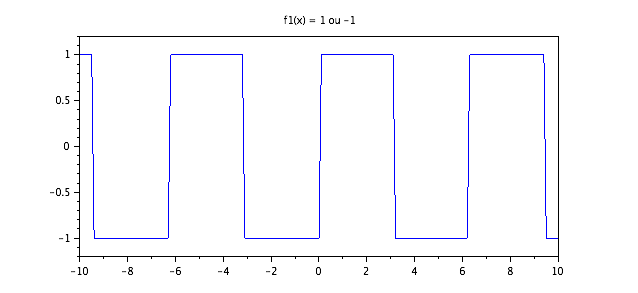
\includegraphics[scale=0.6]{ex1_fig1_0.png}\\*
				\caption{\label{ex1_figure1_0}Courbe de la fonction $f$.}
			\end{figure}\\
			\newpage
			\item Graphe original et ses dix premi\`eres approximations
			\begin{figure}[h!]
				\centering
				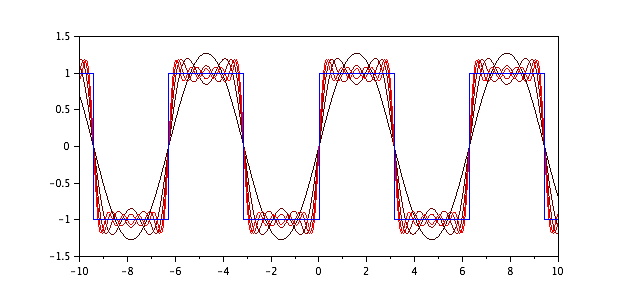
\includegraphics[scale=0.6]{ex1_fig1_1.png}\\*
				\caption{\label{ex1_figure1_1}Courbe de la fonction $f$.}
			\end{figure}\\
		
			\item Richesse fr\'equentielle du signal
			\begin{figure}[h!]
				\centering
				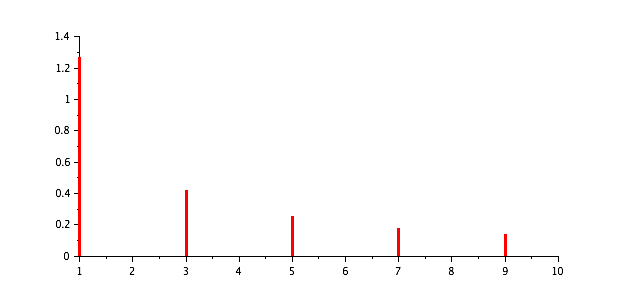
\includegraphics[scale=0.6]{ex1_fig1_2.png}\\*
				\caption{\label{ex1_figure1_2}Richesse du signal $f$.}
			\end{figure}\\
		\end{enumerate}
		\newpage
	
	%2.
		\item $f$ est $2\pi$ p\'eriodique, impaire et vaut $f(x)=x, x \in [0,\pi]$ \\
		\begin{enumerate}
			\item Coefficients de Fourier \\ \\
			Les $a(i)$ \'etant nuls. On obtient ainsi les coefficients suivants pour les $b(i)$ : \\ \\
			\begin{tabular}{l l}
				$b(1) = 2.000000$ & \hspace*{2cm}$b(6) = -0.333333$\\
				$b(2) = -1.000000$ & \hspace*{2cm}$b(7) = 0.285714$\\
				$b(3) = 0.666667$ & \hspace*{2cm}$b(8) = -0.250000$\\
				$b(4) = -0.500000$ & \hspace*{2cm}$b(9) = 0.222222$\\
				$b(5) = 0.400000$ & \hspace*{2cm}$b(10) = -0.200000$\\
			\end{tabular}\\ \\
			\item S\'erie de Fourier
			\begin{figure}[h!]
				\centering
				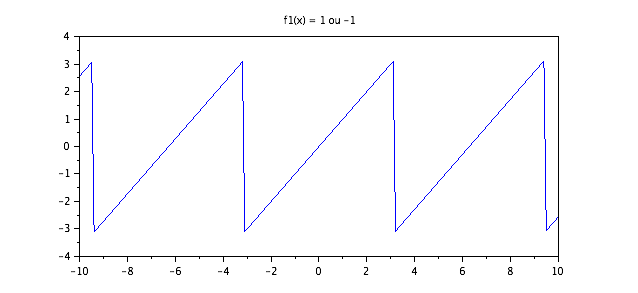
\includegraphics[scale=0.6]{ex1_fig2_0.png}\\*
				\caption{\label{ex1_figure2_0}Courbe de la fonction $f$.}
			\end{figure}\\ 
			\newpage
			\item Graphe original et ses dix premi\`eres approximations
			\begin{figure}[h!]
				\centering
				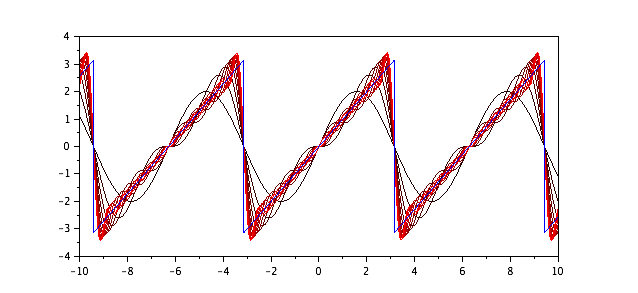
\includegraphics[scale=0.6]{ex1_fig2_1.png}\\*
				\caption{\label{ex1_figure2_1}Courbe de la fonction $f$.}
			\end{figure}\\
		
			\item Richesse fr\'equentielle du signal
			\begin{figure}[h!]
				\centering
				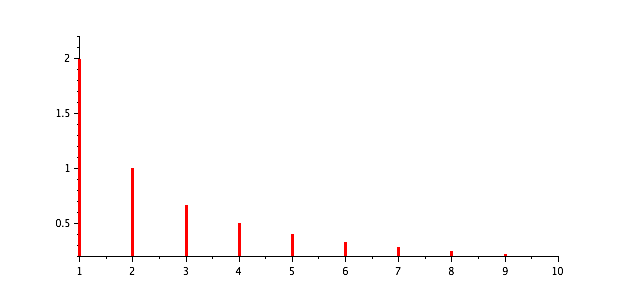
\includegraphics[scale=0.6]{ex1_fig2_2.png}\\*
				\caption{\label{ex1_figure2_2}Richesse du signal $f$.}
			\end{figure}\\
		\end{enumerate}
				\newpage
		
		%3.
		\item $f$ est $2\pi$ p\'eriodique, paire et vaut $f(x)=x, x \in [0,\pi]$ \\
		\begin{enumerate}
			\item Coefficients de Fourier \\ \\
			Les $b(i)$ \'etant nuls. On obtient ainsi les coefficients suivants pour les $a(i)$ : \\ \\
			\begin{tabular}{l l}
				$a(1) = 1.273240$ & \hspace*{2cm}$a(6) = -0.000000$\\
				$a(2) = 0.000000$ & \hspace*{2cm}$a(7) = 0.025984$\\
				$a(3) = 0.141471$ & \hspace*{2cm}$a(8) = 0.000000$\\
				$a(4) = 0.000000$ & \hspace*{2cm}$a(9) = 0.015719$\\
				$a(5) = 0.050930$ & \hspace*{2cm}$a(10) = 0.000000$\\
			\end{tabular}\\
			avec $a(0) = 3.141593$\\ \\
			\item S\'erie de Fourier
			\begin{figure}[h!]
				\centering
				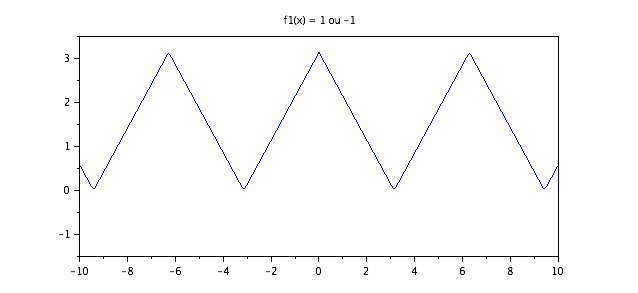
\includegraphics[scale=0.6]{ex1_fig3_0.png}\\*
				\caption{\label{ex1_figure3_0}Courbe de la fonction $f$.}
			\end{figure}\\
			\newpage
			\item Graphe original et ses dix premi\`eres approximations
			\begin{figure}[h!]
				\centering
				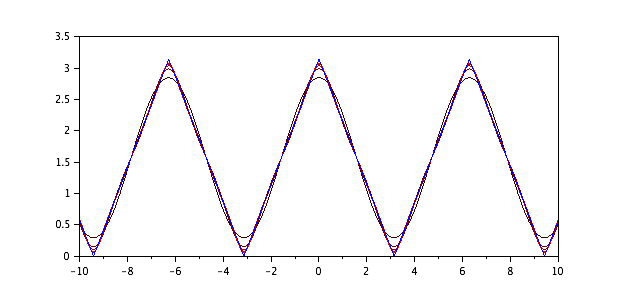
\includegraphics[scale=0.6]{ex1_fig3_1.png}\\*
				\caption{\label{ex1_figure3_1}Courbe de la fonction $f$.}
			\end{figure}\\
		
			\item Richesse fr\'equentielle du signal
			\begin{figure}[h!]
				\centering
				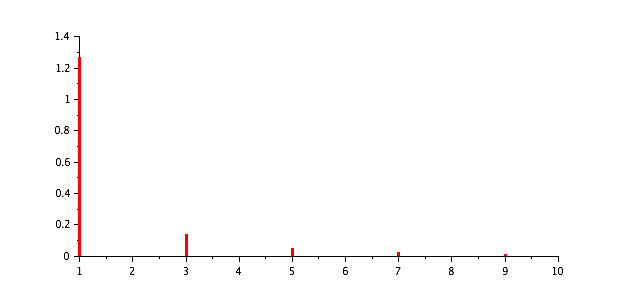
\includegraphics[scale=0.6]{ex1_fig3_2.png}\\*
				\caption{\label{ex1_figure3_2}Richesse du signal $f$.}
			\end{figure}\\
		\end{enumerate}
				\newpage
		
		%4.
		\item $f$ est $2\pi$ p\'eriodique, paire et vaut $f(x)=x^{2}, x \in [0,\pi]$ \\
		\begin{enumerate}
			\item Coefficients de Fourier \\ \\
			Les $b(i)$ \'etant nuls. On obtient ainsi les coefficients suivants pour les $a(i)$ : \\ \\
			\begin{tabular}{l l}
				$a(1) = -4.000000$ & \hspace*{2cm}$a(6) = 0.111111$\\
				$a(2) = 1.000000$ & \hspace*{2cm}$a(7) = -0.081633$\\
				$a(3) = -0.444444$ & \hspace*{2cm}$a(8) = 0.062500$\\
				$a(4) = 0.250000$ & \hspace*{2cm}$a(9) = -0.049383$\\
				$a(5) = -0.160000$ & \hspace*{2cm}$a(10) = 0.040000$\\
			\end{tabular}\\
			avec $a(0) = 6.579736$\\ \\
			\item S\'erie de Fourier
			\begin{figure}[h!]
				\centering
				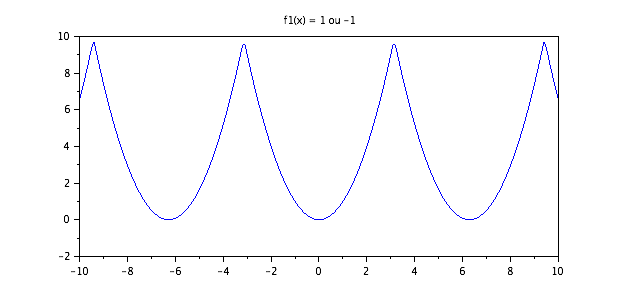
\includegraphics[scale=0.6]{ex1_fig4_0.png}\\*
				\caption{\label{ex1_figure4_0}Courbe de la fonction $f$.}
			\end{figure}\\
			\newpage
			\item Graphe original et ses dix premi\`eres approximations
			\begin{figure}[h!]
				\centering
				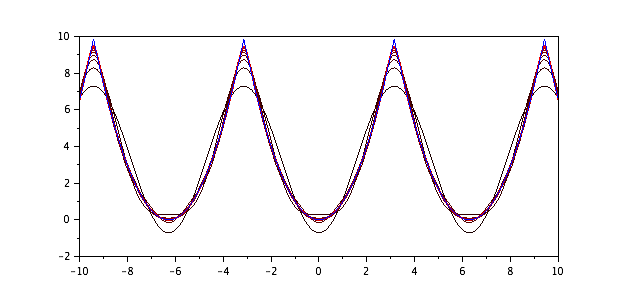
\includegraphics[scale=0.6]{ex1_fig4_1.png}\\*
				\caption{\label{ex1_figure4_1}Courbe de la fonction $f$.}
			\end{figure}\\
		
			\item Richesse fr\'equentielle du signal
			\begin{figure}[h!]
				\centering
				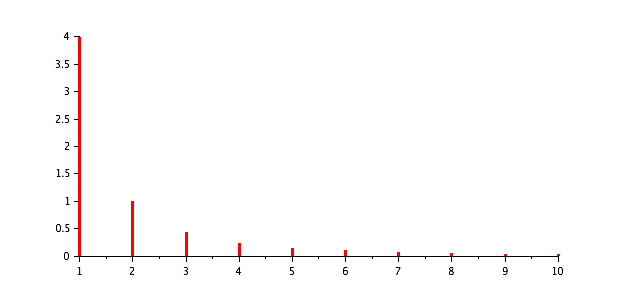
\includegraphics[scale=0.6]{ex1_fig4_2.png}\\*
				\caption{\label{ex1_figure4_2}Richesse du signal $f$.}
			\end{figure}\\
		\end{enumerate}
		\newpage
		
		%5.
		\item $f$ est $2\pi$ p\'eriodique, impaire et vaut $f(x)=x(\pi + |x|), x \in [-\pi,\pi]$ \\
		\begin{enumerate}
			\item Coefficients de Fourier \\ \\
			Les $a(i)$ \'etant nuls. On obtient ainsi les coefficients suivants pour les $b(i)$ : \\ \\
			\begin{tabular}{l l}
				$b(1) = 2.546479$ & \hspace*{2cm}$b(6) = 0.000000$\\
				$b(2) = 0.000000$ & \hspace*{2cm}$b(7) = 0.007424$\\
				$b(3) = 0.094314$ & \hspace*{2cm}$b(8) = -0.000000$\\
				$b(4) = -0.000000$ & \hspace*{2cm}$b(9) = 0.003493$\\
				$b(5) = 0.020372$ & \hspace*{2cm}$b(10) = -0.000000$\\
			\end{tabular}\\ \\
			\item S\'erie de Fourier
			\begin{figure}[h!]
				\centering
				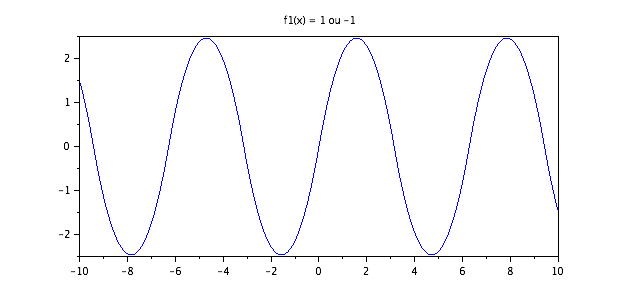
\includegraphics[scale=0.6]{ex1_fig5_0.png}\\*
				\caption{\label{ex1_figure5_0}Courbe de la fonction $f$.}
			\end{figure}\\
			\newpage
			\item Graphe original et ses dix premi\`eres approximations
			\begin{figure}[h!]
				\centering
				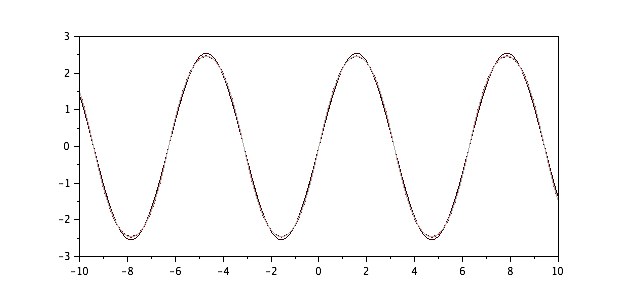
\includegraphics[scale=0.6]{ex1_fig5_1.png}\\*
				\caption{\label{ex1_figure5_1}Courbe de la fonction $f$.}
			\end{figure}\\
		
			\item Richesse fr\'equentielle du signal
			\begin{figure}[h!]
				\centering
				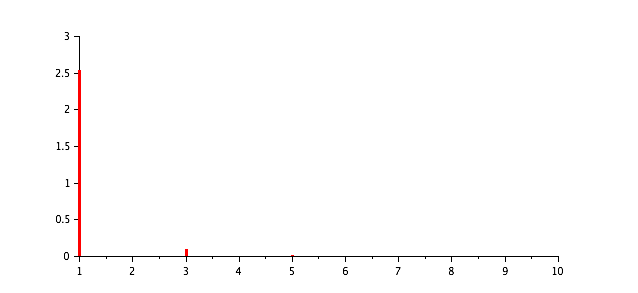
\includegraphics[scale=0.6]{ex1_fig5_2.png}\\*
				\caption{\label{ex1_figure5_2}Richesse du signal $f$.}
			\end{figure}\\
		\end{enumerate}

		
	\end{enumerate}
\newpage



	

%Exercice 2
\chapter{\'Etude de fonctions}
% 1
	\begin{enumerate}
	\item \[f(x)=(sin\,x)^{1/3}\]
	La fonction f est d\'efinie sur l'intervalle ($-\pi;\pi$). Elle est compos\'ee d'une fonction sinus, ce qui la rend impaire. Elle n'admet aucune valeur interdite et on a $f(0^+)=f(0^-)=\sqrt{0}=0$. Elle est donc continue.
	\begin{figure}[h!]
		\centering
		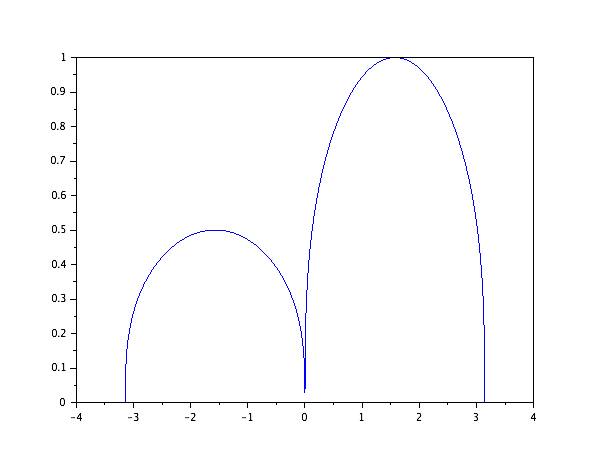
\includegraphics[scale=0.6]{ex2_fig1.png}
		\caption{\label{figure1}Courbe de la fonction $f$.}
		\end{figure}
		\\
	Sa d\'eriv\'ee est \[f'(x)=\frac{1}{3} cos x (sin\,x)^{-2/3}\] Elle admet une asymptote verticale en $0$ et n'est donc pas continue.
	La fonction $f$ est continue mais non d\'erivable sur ($-\pi;\pi$).
	% Faut-il ajouter le programme Scilab ? Que veux dire "Commenter" ?
	\newpage
% 2
	\item \[f(x)=(sin\,x)^{4/3}\]
	La fonction f est d\'efinie sur l'intervalle ($-\pi;\pi$). Elle n'admet aucune valeur interdite et on a $f(0^+)=f(0^-)=\sqrt[3]{0}=0$. Elle est donc continue.
	\begin{figure}[h!]
		\centering
		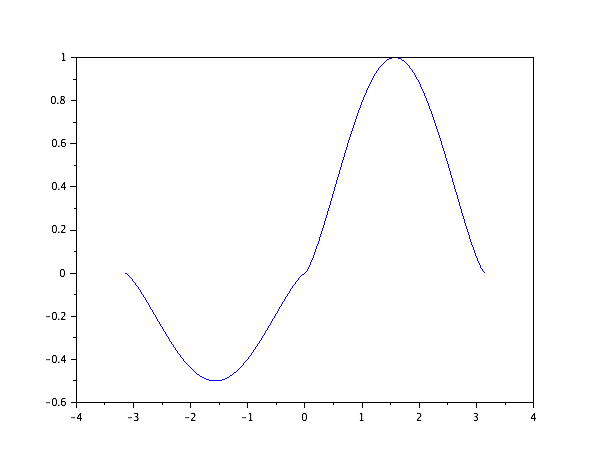
\includegraphics[scale=0.6]{ex2_fig2.png}
		\caption{\label{figure2}Courbe de la fonction $f$.}
		\end{figure}
		\\
	Sa d\'eriv\'ee est \[f'(x)=\frac{4}{3} cos\,x (sin\,x)^{1/3}\] Elle n'admet pas d'asymptote et est donc continue.
	La fonction $f$ est continue et d\'erivable, donc r\'eguli\`ere.
	\newpage
% 3
	\item \[f(x)=
  \left\{
      \begin{aligned}
        cos\,x\quad , si\quad x > 0\\
        -cos\,x\quad ,si\quad x \le 0\\
      \end{aligned}
    \right.\]
	La fonction f est d\'efinie sur l'intervalle ($-\pi;\pi$). Elle n'admet aucune valeur interdite et on a $f(0^+)=1$ et $f(0^-)=-1$. Elle n'est donc pas continue en 0.
	\begin{figure}[h!]
		\centering
		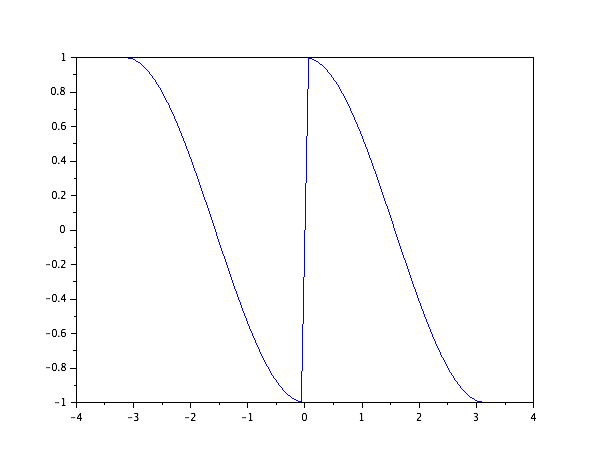
\includegraphics[scale=0.6]{ex2_fig3.png}
		\caption{\label{figure3}Courbe de la fonction $f$.}
		\end{figure}
		\\
	Elle est d\'erivable par morceaux et sa d\'eriv\'ee est \[f'(x)=
  \left\{
      \begin{aligned}
        -sin\,x\quad , si\quad x > 0\\
        sin\,x\quad ,si\quad x \le 0\\
      \end{aligned}
    \right.\] \\
	La fonction $f$ est continue par morceaux et d\'erivable par morceaux, donc r\'eguli\`ere par morceaux.
	\newpage
% 4
	\item \[f(x)=
  \left\{
      \begin{aligned}
        sin\,x\quad , si\quad x > 0\\
        -sin\,2x\quad ,si\quad x \le 0\\
      \end{aligned}
    \right.\]
	La fonction f est d\'efinie sur l'intervalle ($-\pi;\pi$). Elle n'admet aucune valeur interdite et on a $f(0^+)=f(0^-)=0$. Elle est donc continue.
	\begin{figure}[h!]
		\centering
		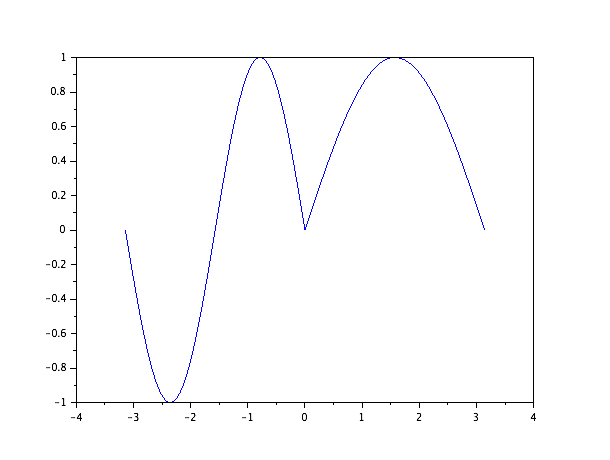
\includegraphics[scale=0.6]{ex2_fig4.png}
		\caption{\label{figure4}Courbe de la fonction $f$.}
		\end{figure}
		\\
	Elle est d\'erivable par morceaux et sa d\'eriv\'ee est \[f'(x)=
  \left\{
      \begin{aligned}
        cos\,x\quad \;, si\quad x > 0\\
        -2cos\,2x\quad ,si\quad x \le 0\\
      \end{aligned}
    \right.\]
	La fonction $f$ est continue et d\'erivable par morceaux, donc r\'eguli\`ere par morceaux.
	\newpage
% 5
	\item \[f(x)=
  \left\{
      \begin{aligned}
        (sin\,x)^{1/5}\;\; , si\quad x < \pi/2\\
        -cos\,x\quad \;,si\quad x \ge \pi/2\\
      \end{aligned}
    \right.\]
	La fonction f est d\'efinie sur l'intervalle ($-\pi;\pi$). Elle n'admet aucune valeur interdite et on a $f(0^+)=f(0^-)=\sqrt{0}=0$ et $f(\pi/2)=0$ et $\lim\limits_{\substack{x \rightarrow \pi/2 \\ x<\pi/2}} f(x) = 1$. Elle est continue en 0 mais pas en $\pi/2$, elle est donc continue par morceaux.
	\begin{figure}[h!]
		\centering
		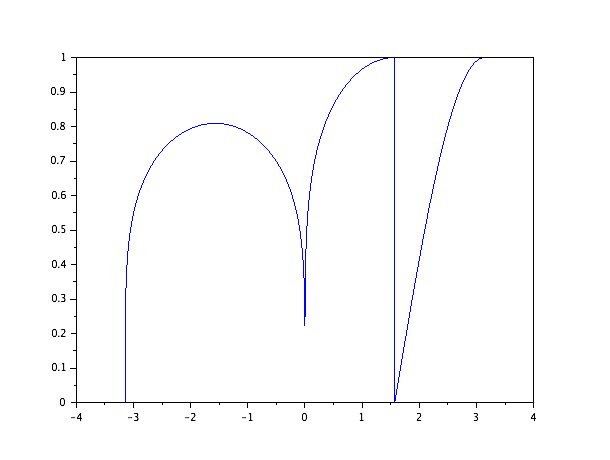
\includegraphics[scale=0.6]{ex2_fig5.png}
		\caption{\label{figure5}Courbe de la fonction $f$.}
		\end{figure}
		\\
	Elle est d\'erivable par morceaux et sa d\'eriv\'ee est \[f'(x)=
  \left\{
      \begin{aligned}
        \frac{1}{5}cos\,x\,(sin\,x)^{1/5}\quad , si\quad x < \pi/2\\
        sin\,x\qquad \qquad ,si\quad x \ge \pi/2\\
      \end{aligned}
    \right.\]
	La fonction $f$ est continue par morceaux et d\'erivable par morceaux, donc r\'eguli\`ere par morceaux.
	\end{enumerate}
	
%Exercice 3
\chapter{Ph\'enom\`ene de Gibbs}
\section{Historique}

Lors de l'\'etude des s\'eries de Fourier et des transform\'ees de Fourier, il appara\^it parfois une d\'eformation du signal, connue sous le nom de ph\'enom\`ene de Gibbs. Ce ph\'enom\`ene est un effet de bord qui se produit \`a proximit\'e d'une discontinuit\'e, lors de l'analyse d'une fonction d\'erivable par morceaux.
Le ph\'enom\`ene fut mis pour la premi\`ere fois en \'evidence en 1848 par Henry Wilbraham, mais cette d\'ecouverte ne connut gu\`ere d'\'echo.

En 1898, Albert Michelson d\'eveloppa un syst\`eme m\'ecanique capable de calculer et sommer la s\'erie de Fourier d'un signal donn\'e en entr\'ee. Il observa alors un effet d'amplification des discontinuit\'es, qui persistait malgr\'e l'augmentation du nombre de coefficients calcul\'es.

Alors que Michelson soup�onnait un d\'efaut dans la fabrication de son engin, Josiah Willard Gibbs montra que le ph\'enom\`ene \'etait d'origine math\'ematique et se produisait dans des conditions tr\`es g\'en\'erales. En 1906, Maxime B\^ocher donna la premi\`ere interpr\'etation satisfaisante du ph\'enom\`ene auquel il donna le nom de ph\'enom\`ene de Gibbs.

Le ph\'enom\`ene de Gibbs est, en quelque sorte, un\og d\'efaut d'approximation \fg  pour une fonction continue de classe $C^1$ par morceaux. 

\section{D\'emonstration}
Soit f la fonction 2$\pi$-p\'eriodique et impaire telle que $f(x) = 1$ sur $[0; \pi]$.\\

Nous allons montrer que \[S_{f(x)}=\frac{4}{\pi}\sum\limits_{n=0}^{\infty}\frac{sin(2k-1)}{2k-1}\]

Nous savons que $S_{f(x)}=\displaystyle\sum\limits_{n=0}^{\infty} b_{n}sinnx$, car f est impaire.\\
Or, 
\begin{eqnarray*}
b_{n}&=&\frac{1}{\pi}\int_{-\pi}^{\pi}f(x)sinnx\\
		 &=&\frac{1}{\pi}\int_{-\pi}^{0}f(x)sinnx\,+\,\frac{1}{\pi}\int_{0}^{\pi}f(x)sinnx\\
		 &=&-\frac{1}{\pi}\int_{-\pi}^{0}sinnx\,+\,\frac{1}{\pi}\int_{0}^{\pi}sinnx\\
		 &=&\frac{1}{\pi}\int_{0}^{\pi}sinnx\,+\,\frac{1}{\pi}\int_{0}^{\pi}sinnx\\
		 &=&\frac{2}{\pi}\int_{0}^{\pi}sinnx\\
		&=&\frac{2}{\pi}\left[\frac{-cosnx}{k}\right]_0^\pi\\
		 &=&\frac{2}{\pi}\left(-\frac{cosn\pi}{n}+\frac{1}{n}\right)\\
		 &=&\frac{2}{\pi}\left(-\frac{cosn\pi}{n}+\frac{1}{n}\right)\\
	\end{eqnarray*}
D'o\`u 
\begin{eqnarray*}
S_{f(x)}&=&\frac{2}{\pi}\displaystyle\sum\limits_{n=0}^{\infty}\frac{1-cosn\pi}{n}sinnx\\
		&=&\frac{2}{\pi}\displaystyle\sum\limits_{n=0}^{\infty}\frac{1-(-1)^{n}}{n}sinnx\\
		&=&\frac{2}{\pi}\sum\limits_{n\,pair}^{\infty}\frac{1-(-1)^{n}}{n}sinnx\,+\,\frac{2}{\pi}\sum\limits_{n\,impair}^{\infty}\frac{1-(-1)^{n}}{n}sinnx\\
		&=&\frac{4}{\pi}\sum\limits_{n\,impair}^{\infty}\frac{sinnx}{n}\\
		&=&\frac{4}{\pi}\sum\limits_{n=1}^{\infty}\frac{sin(2k-1)x}{2k-1}\qquad,\;\text{o\`u}\;n=2k-1\;,\;k\,\in\,\pmb{\mathbb{R}}\\
	\end{eqnarray*}
\section{Approximations de Fourier}
\begin{enumerate}
	\item Approximation pour n = 2
		\begin{figure}[h!]
		\centering
		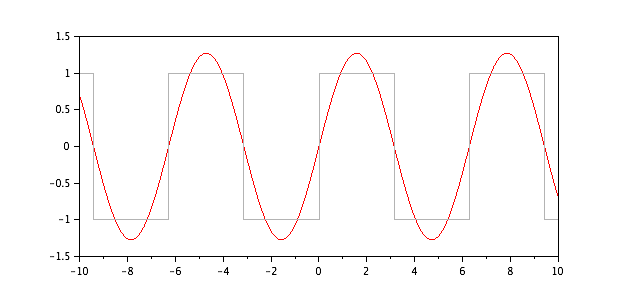
\includegraphics[scale=0.6]{ex3_figN2.png}
		\caption{\label{ex3figN2}Courbe de la fonction $f$ pour n = 2.}
		\end{figure}
		\newpage

	\item Approximation pour n = 5
		\begin{figure}[h!]
		\centering
		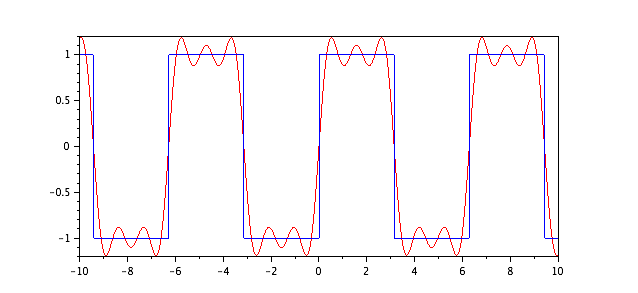
\includegraphics[scale=0.6]{ex3_figN5.png}
		\caption{\label{ex3figN5}Courbe de la fonction $f$ pour n = 5.}
		\end{figure}
		
	\item Approximation pour n = 10
		\begin{figure}[h!]
		\centering
		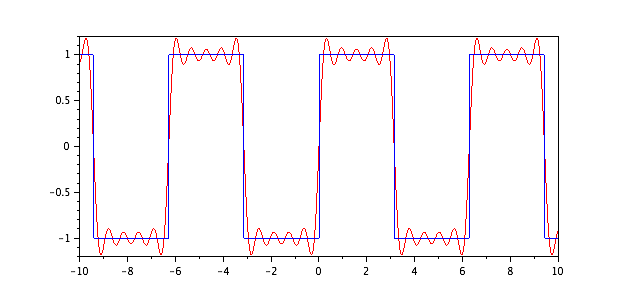
\includegraphics[scale=0.6]{ex3_figN10.png}
		\caption{\label{ex3figN10}Courbe de la fonction $f$ pour n = 10.}
		\end{figure}
		\newpage

	\item Approximation pour n = 20
		\begin{figure}[h!]
		\centering
		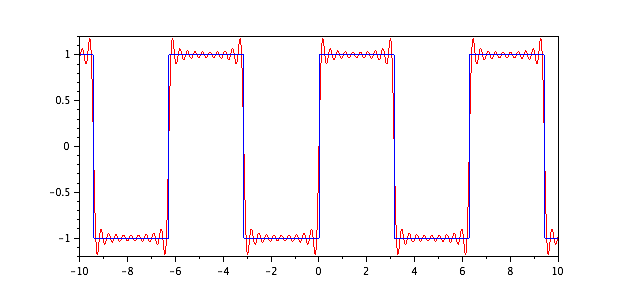
\includegraphics[scale=0.6]{ex3_figN20.png}
		\caption{\label{ex3figN20}Courbe de la fonction $f$ pour n = 20.}
		\end{figure}
		
	\item Approximation pour n = 60
		\begin{figure}[h!]
		\centering
		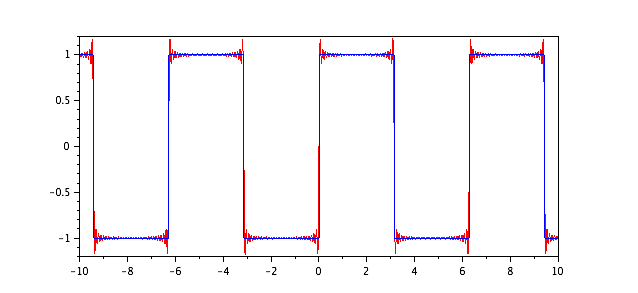
\includegraphics[scale=0.6]{ex3_figN60.png}
		\caption{\label{ex3figN60}Courbe de la fonction $f$ pour n = 60.}
		\end{figure}\\

On remarque donc qu'au voisinage d'une discontinuit\'e une bosse apparait. Or quand $n$ augmente cette derni\`ere subsiste de part et d'autre d'une discontinuit\'e. Pla\c cons nous alors \`a droite du point de discontinuit\'e $0$ par exemple. On note que lorsque $n$ augmente, le point en lequel il y a un pic s'approche de $0$, mais la hauteur reste constante. Nous allons essayer d'expliquer ce ph\'enom\`ene dans la partie suivante.
\end{enumerate}
\newpage
\section{Explication du ph\'enom\`ene}
	\subsection{Contexte}
Soit $f$ la fonction $2\pi$-p\'eriodique et impaire telle que $f(x) = 1$ sur $[0; \pi]$.\\

On note que la fonction pr\'esente une discontinuit\'e en tout point multiple de $\pi$. La limite \`a droite et la limite \`a gauche en ces points vaut +1 et -1. De plus en dehors de ces points la fonctions est continue. Nous avons donc une fonction continue par morceau et sa d\'eriv\'ee l'est \'egalement. Ainsi on peut dire que $f$ est $C^{1}$ par morceaux
	\subsection{Analyse Math\'ematique}
		\subsubsection{Application du Th\'eor\`eme de Dirichlet}
Comme f est impaire on a donc :

\[S_{f(x)}=\frac{4}{\pi}\sum\limits_{k=1}^{\infty}\frac{sin(2k-1)x}{2k-1}\qquad,\;\text{o\`u}\;k\,\in\,\pmb{\mathbb{R}}\]


Pour une fonction $C^{1}$ par morceaux, le th\'eor\`eme de Dirichlet nous indique quel est la limite de ces sommes partielles. Si l'on consid\`ere un point de continuit\'e de la fonction, ces sommes partielles vont converger vers $f(x)$.  Ainsi au point de discontinuit\'e ($x=0$), la limite de ces sommes partielles va \^etre la demi-somme entre la limite \`a droite et la limite \`a gauche de la valeur de la fonction au point consid\'erer\'e. Ici, la demi-somme vaut $0$ :\\


\[S_{f(x)}=\frac{4}{\pi}\sum\limits_{k=1}^{\infty}\frac{sin(2k-1)x}{2k-1} \left\vert{_{x=0}}\right. = \frac{1}{2}[+1+(-1)] = 0\]\\

En particulier, sur un tel point la limite ne vaut pas la valeur du signal $f(0)=1$, alors que la demi-somme vaut $0$

On s'int\'eresse par la suite au comportement au voisinage du point de discontinuit\'e.

		\subsubsection{Comportement au voisinage d'un point de discontinuit\'e}

\'Etudions la somme partielle $S_{p}(x)$:\\
Calculons sa d\'eriv\'ee afin d'\'etablir son tableaux de variations. \\
Comme $\displaystyle\frac{d}{dt}sin((2k-1)x) = (2k-1)cos((2k-1)x)$ on d\'eduit que \\
$$\frac{d}{dt}S_{p}(x) = \frac{4}{\pi}\sum\limits_{k=1}^{\infty}cos((2k-1)x)$$\\

Ensuite on pose : \[cos((2k-1)x) = Re [e^{i(2k-1)x}] \quad \text{et} \quad \sum\limits_{k=0}^{n}q^{k} = \frac{1-q^{n+1}}{1-q}\]

On d\'eduit l'expression suivante :
\[ 
\left\{
  \begin{aligned}
  \frac{d}{dt}S_{p}(x)= \frac{2}{\pi}\frac{sin(2kx)}{sin(x)}\quad \text{, pour} \quad t \neq 0\\
  \frac{d}{dt}S_{p}(x)= \frac{4}{\pi} \quad \text{, par calcul direct}\\
  \end{aligned}
\right.\]
Par int\'egration on doit obtenir une expression explicite de $S_{p}(x)$. Or comme somme de sinus elle s'annule en $x=0$ on prend donc cette primitive qui s'annule en 0 :
$$S_{p}(x)= \frac{2}{\pi}\int_{0}^{x}\frac{sin(2pu)}{sin(u)} \, \mathrm{d}u$$

Afin d'\'etudier la fonction $S_{p}(x)= \frac{2}{\pi}\int_{0}^{x}\frac{sin(2pu)}{sin(u)} \, \mathrm{d}u$ on dresse son tableau de variation.\\
Cherchons les valeurs qui annulent cette d\'eriv\'e.\\
Soit $x \in [0,\pi]$ tels que $S_{p}^{'}(x) = \frac{d}{dt}S_{p}(x) = \frac{2}{\pi}\frac{sin(2pu)}{sin(u)} = 0$. On obtient les z\'eros de la d\'eriv\'e suivants : \[sin(2px)=0 \iff 2px = 0[\pi]\]
\newpage

Donc pour $x \in ]0,\pi[$  \[S_{p}^{'}(x) = 0 \iff x \in \left\{\frac{\pi}{2p},\frac{2\pi}{2p},...,\frac{(2p-1)\pi}{2p}\right\}\]
D'o\`u la racine la plus proche \`a droite de $x = 0$ est $x_{1} = \frac{\pi}{2p}$. On va par la suite \'etudier les variations de $S_{p}(x)$ au voisinage de ce point :\\


\begin{tikzpicture}
\tkzTabInit{$x$/1,$S_{p}^{'}(x)$/1,$S_{p}(x)$/2}{$0$,$\frac{\pi}{2p}$,$\frac{2\pi}{2p}$}
\tkzTabLine{d,+,z,-,z,}
\tkzTabVar{D-/$0$,+/$m_{1,p}$,-/$m_{2,p}$}
\end{tikzpicture}\\

Ce qui correspond \`a la courbe \ref{ex3figN5}

		\subsubsection{Valeur et amplitude de la bosse de Gibbs}
Valeur du maximal local :
\[m_{1,p} = S_{p}(\frac{\pi}{2p}) = \frac{2}{\pi}\int_{0}^{\frac{\pi}{2p}}\frac{sin(2pu)}{sin(u)} \, \mathrm{d}u\]
On effectue le changement de variable suivant : $v = 2pu$, ce qui donne :
\[m_{1,p} = \frac{2}{\pi}\int_{0}^{\pi}\frac{sin(v)}{sin(\frac{v}{2p})} \frac{dv}{2p}\]
Apr\`es transformation on obtient :
\[m_{1,p} = \frac{2}{\pi}\int_{0}^{\pi}\frac{sin v}{v}\frac{1}{\frac{sin(\frac{v}{2p})}{\frac{v}{2p}}} dv\]
Par ailleurs on sait que :\\
\begin{equation}
\left\{ \,
  \begin{aligned}
  \lim\limits_{p \rightarrow +\infty} \frac{v}{2p} \rightarrow 0\\
  \lim\limits_{h \rightarrow 0} \frac{sin h}{h} = 1\\
  \end{aligned}
\right
\label{indice1}
\end{equation}
\newpage

On cherche donc la limite suivante :\\
\[\lim\limits_{p \rightarrow +\infty} m_{1,p} = \frac{2}{\pi} \lim\limits_{p \rightarrow +\infty} \int_{0}^{\pi}\frac{sin v}{v}\frac{1}{\frac{sin(\frac{v}{2p})}{\frac{v}{2p}}}dv\]

On fait rentrer la limite \`a l'int\'erieur de l'int\'egrale car $f$ est $C^{1}$ :\\
\[\frac{2}{\pi} \lim\limits_{p \rightarrow +\infty} \int_{0}^{\pi}\frac{sin v}{v}\frac{1}{\frac{sin(\frac{v}{2p})}{\frac{v}{2p}}}dv = \frac{2}{\pi} \int_{0}^{\pi} \lim\limits_{p \rightarrow +\infty} \bigg[\frac{sin v}{v}\frac{1}{\frac{sin(\frac{v}{2p})}{\frac{v}{2p}}}\bigg]dv\]
 D'apr\`es le point \eqref{indice1}\ on a le r\'esultat suivant :
 \[\frac{2}{\pi} \int_{0}^{\pi} \lim\limits_{p \rightarrow +\infty} \bigg[\frac{sin v}{v}\frac{1}{\frac{sin(\frac{v}{2p})}{\frac{v}{2p}}}\bigg]dv = \frac{2}{\pi} \int_{0}^{\pi}\frac{sin v}{v}dv\]

		\subsubsection{Conclusion}
A partir de ce point nous pouvons calculer num\'eriquement le r\'esultat suivant :
$$\frac{2}{\pi} \int_{0}^{\pi}\frac{sin v}{v}dv = 1.18 = 1 + 0.18$$\\
La bosse d\'epasse donc toujours la valeur 1 de la fonction au voisinage de 0 d'une quantit\'e incompressible 0.18. L'amplitude de la bosse est donc toujours sup\'erieur \`a 0.18 pour notre fonction.\\
La g\'en\'eralisation de notre fonction (non abord\'e ici) montre que la bosse de Gibbs a une hauteur proportionnelle \`a une amplitude du saut de discontinuit\'e. Ce coefficient de proportionnalit\'e universel est appel\'e coefficient de Wilbraham Gibbs est vaut 9\% du saut.


%Exercice 4
\chapter{Application des s\'erie de Fourier}
\section{La corde pinc\'ee}
\section{La corde frapp\'ee}

%Exercice 5
\chapter{Equation de la chaleur}

%Compl\'ement au TP
\chapter{Compl\'ements}
\section{Finance}
\section{Informatique}

%Test de texte
Comme le disait Jean de la Fontaine dans sa fable :
\begin{quote}
Rien de sert de courir, il faut partir à point.
\end{quote}


\end{document}